\section{Casos de éxito}
Tal crecimiento sin precedentes de la IoT, los dispositivos de interacción y la adopción de la computación móvil requiere marcos de toma de decisiones y computación basados en datos inteligentes para abstraer estos datos de sensores sin procesar, heterogéneos pero complementarios, en información procesable y conocimiento significativo. Los últimos años han visto un tremendo crecimiento en la investigación de IA que, en parte, ha sembrado e impulsado el surgimiento de varios servicios cognitivos como dominio mediador entre la IA y los datos de IoT para aprovechar y desplegar la riqueza de la información para lograr la naturalidad y la sincronicidad de los medios.
Por ello se tiene que los servicios cognitivos se pueden agrupar en términos generales en cinco categorías: lenguaje, habla, visión, conocimiento y búsqueda. Los ejemplos de cada categoría incluyen: 1) los servicios lingüísticos se denominan reconocimiento y vinculación de entidades, análisis de opiniones y clasificación de intenciones; 2) servicios de voz tales como conversión de voz a texto y viceversa; 3) servicios de visión, por ejemplo, reconocimiento facial y subtítulos automáticos de imágenes; 4) conocimientos tales como análisis de datos y descubrimiento de noticias; y 5) búsqueda como sugerencia automática, imagen, noticias, video y búsqueda web.  Figura 2 muestra
 cómo un chatbot básico se puede ampliar con varios servicios cognitivos en línea para lograr una inteligencia similar a la humana. Si bien los servicios Cognitivos de Watson de IBM se muestran en estos ejemplos, ahora hay disponibles conjuntos crecientes de servicios alternativos \cite{Molnar2019}.

\begin{figure}[htbp]
\centerline{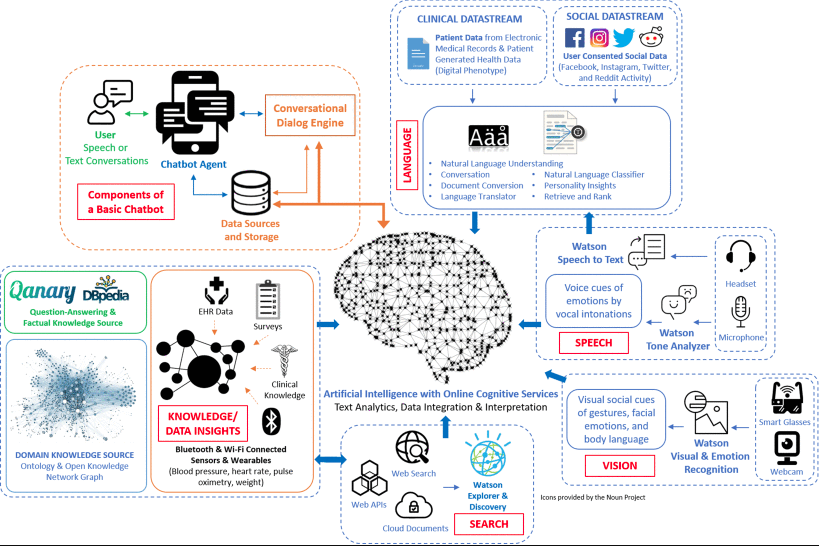
\includegraphics[width = 0.5 \textwidth]{fig02.png}}
\caption{Ilustración de cómo se puede ampliar un chatbot básico utilizando un conjunto de servicios cognitivos de ejemplo.}
\label{fig2}
\end{figure}
{\color{red}}

Las principales empresas tecnológicas (Amazon, Facebook e IBM) se han embarcado en el uso de la tecnología de voz. Si bien el éxito hasta ahora es modesto, las conversaciones de voz atractivas (en lugar de texto) en el chatbot son una promesa importante para la futura interacción hombre-máquina. Si bien los chatbots contemporáneos de propósito general han tenido un éxito limitado principalmente debido a la fragilidad en el contexto del modelado y la capacidad de utilizar un conocimiento más amplio, los chatbots en un dominio como el de la atención médica son muy prometedores y están recibiendo un gran interés correspondiente. Esto se debe en parte a la capacidad de utilizar datos multimodales y el acceso al conocimiento estructurado de la medicina, como lo demuestran las aplicaciones digitales de salud personalizadas para el asma y las enfermedades cardiovasculares. [9] , [10]Con el uso de IoT ampliado con un conjunto de servicios cognitivos, como se ilustra en la Figura 2 , para proporcionar el contexto circundante, las conversaciones de chatbot se pueden hacer más sólidas y significativas. La siguiente sección ilustra cómo los servicios cognitivos en línea pueden aprovechar los datos multimodales para brindar acceso e integración con los dominios de atención médica \cite{Majarres}.

\subsection{Integracin con dominios de salud}

Si bien la alimentación de datos sin procesar generados a partir de IoT en varias canalizaciones de servicios cognitivos en línea para traducirlos en información significativa es un paso más cerca de los chatbots inteligentes, creemos que también es importante que el sistema combine, desmitifique y dé sentido a estos datos a través de la contextualización, personalización y abstracción. Contextualización se refiere a la interpretación de datos en términos de conocimiento (contexto). Por lo general, se refiere al mapeo de datos detallados que cubren varias facetas mediante la determinación del tipo y el valor de los datos, y luego los ubica en relación con otros conceptos de dominio, lo que deriva en una interpretación significativa de los resultados. Como ejemplo, un chatbot contextualizado con conocimiento del dominio puede comprender los términos de la jerga que se usan comúnmente en las redes sociales, como "bupe", que se refiere a su jerga médica "buprenorfina" \cite{Rojas}. Personalización se refiere al curso de acción futuro teniendo en cuenta varios factores con respecto a un paciente en particular, como el historial de salud, las características físicas, el entorno, la actividad y el estilo de vida. Por ejemplo, un chatbot contextualizado y personalizado puede indicar el clima con respecto a la vulnerabilidad de un paciente asmático a un alto nivel de polen de ambrosía y sugerir acciones apropiadas. Abstracciónes una técnica computacional que mapea y asocia datos sin procesar con información relacionada con la acción para proporcionar una vista integrada de las medidas de remediación adecuadas. Por ejemplo, una alta actividad diaria en el contexto de la salud puede abstraerse y traducirse en un bajo riesgo de problemas cardíacos según la información demográfica y genética, así como la dieta. Para pintar una perspectiva más granular, a continuación se ilustran algunos casos de uso sobre cómo estos chatbots inteligentes que aprovechan los servicios cognitivos en línea se pueden usar como un "entrenador de salud personal" en los dominios de atención médica.

Como instancias de chatbots inteligentes creados con servicios cognitivos, describimos tres chatbots inteligentes en desarrollo en proyectos financiados por NIH sobre depresión/salud mental ( http://bit.ly/depression-social ), asma pediátrica ( http://bit.ly /kSalud-Asma), y cuidado de ancianos. En el caso de la enfermedad mental, la detección convencional a menudo administra Cuestionarios de Salud del Paciente (PHQ-9) para evaluar la gravedad de la depresión del paciente. Sin embargo, tal cribado tiene dos defectos inherentes. Se basa en gran medida en la capacidad del paciente para recordar eventos que ocurrieron durante las últimas dos semanas, y todos los criterios del PHQ-9 tienen el mismo peso. Por ejemplo, el criterio “sentirse cansado o tener poca energía” se pondera de manera similar a los “pensamientos de que estaría mejor muerto o lastimarse a sí mismo de alguna manera”. Un chatbot inteligente tiene la capacidad de aprovechar varios dispositivos IoT y servicios cognitivos en línea, como una cámara para evaluar el estado de ánimo actual de un paciente a través del reconocimiento visual; el micrófono que aprovecha el servicio de analizador de tono para analizar la tonalidad y el sentimiento del habla; servicio de insights de personalidad para determinar la personalidad del paciente; acceso a los perfiles consentidos del paciente para descubrir manifestaciones de comportamiento y calumnias en varias plataformas de redes sociales; comprensión de idiomas y servicios de traducción para el análisis lingüístico, como el uso de términos de argot; y QnA maker para formular preguntas inteligentes. Una combinación de estos servicios cognitivos en línea puede superar la naturaleza transitoria del recuerdo de la memoria y capturar cambios de comportamiento sutiles que de otro modo se pasarían por alto o no se traducirían de manera evidente durante la evaluación de PHQ-9. Estos permiten además una entrada viable para la entrega de psicoterapia de acuerdo con la terapia cognitivo-conductual. comprensión de idiomas y servicios de traducción para el análisis lingüístico, como el uso de términos de argot; y QnA maker para formular preguntas inteligentes. Una combinación de estos servicios cognitivos en línea puede superar la naturaleza transitoria del recuerdo de la memoria y capturar cambios de comportamiento sutiles que de otro modo se pasarían por alto o no se traducirían de manera evidente durante la evaluación de PHQ-9. Estos permiten además una entrada viable para la entrega de psicoterapia de acuerdo con la terapia cognitivo-conductual. comprensión de idiomas y servicios de traducción para el análisis lingüístico, como el uso de términos de argot; y QnA maker para formular preguntas inteligentes. Una combinación de estos servicios cognitivos en línea puede superar la naturaleza transitoria del recuerdo de la memoria y capturar cambios de comportamiento sutiles que de otro modo se pasarían por alto o no se traducirían de manera evidente durante la evaluación de PHQ-9. Estos permiten además una entrada viable para la entrega de psicoterapia de acuerdo con la terapia cognitivo-conductual.[11] e iniciar la necesidad de una intervención de tratamiento conforme a los protocolos médicos.

En el caso de la enfermedad del asma, el diagnóstico tradicional, como la prueba de control del asma, generalmente se centra y se limita a la información disponible del paciente al médico en el momento de las visitas al hospital. Hay tantos conocimientos que se pueden obtener de datos tan limitados. Un chatbot inteligente, por el contrario, es capaz de llenar y cerrar este vacío de información. Por ejemplo, puede aprovechar los servicios en línea para datos meteorológicos y registros médicos electrónicos (analizados mediante servicios cognitivos como conversión de documentos, clasificación y comprensión del lenguaje natural) para comprender la susceptibilidad del paciente al polen de ambrosía, combinar estos tipos individuales de información y sugerir cursos apropiados. de acciones Imagine dos respuestas diferentes para la misma consulta que busca información meteorológica, “Puede esperar un clima bastante soleado hoy” y “Puede esperar un clima bastante soleado hoy, sin embargo, el nivel de polen de ambrosía es un poco alto, lo que no parece bueno para su condición de asma. Minimice cualquier actividad al aire libre”. La primera es una tarea de recuperación de información sin capacidad cognitiva, mientras que la segunda representa capacidades de razonamiento contextualizado, inferencia y recomendación que pueden enriquecer la calidad de vida del paciente.

En el caso del cuidado de ancianos, además de residir con un mayor riesgo de desarrollar enfermedades crónicas, los residentes mayores a menudo caen en los grupos de analfabetos y escépticos tecnológicos en comparación con sus compatriotas más jóvenes ( http://bit.ly/Elder-Technology). Un chatbot proporciona una barrera de entrada más baja para los ancianos que adoptan el uso de la tecnología. Como ejemplo ortogonal, un chatbot equipado con reconocimiento de voz, traducción multilingüe y servicios cognitivos de comprensión del lenguaje natural permite a las personas mayores con problemas de alfabetización enviar mensajes de texto o hablar, lo que sea con lo que se sientan más cómodos. Alternativamente, un chatbot con acceso a API geográficas, locales y web también es capaz de brindar apoyo social, como organizar sesiones de telesalud, programar citas médicas y coordinar y organizar servicios de transporte para personas mayores con discapacidades físicas y barreras de transporte, especialmente en ciudades congestionadas. Sin embargo, tales capacidades y funcionalidades ilustradas solo han arañado la superficie de los posibles casos de uso más amplios de servicios cognitivos en línea para chatbots inteligentes. Su impacto emergente y su perfecta integración en la prestación de atención médica para una salud personalizada aumentada[12] tales como el autocontrol, la autoevaluación, el autocontrol, la intervención y la proyección del riesgo y la progresión de la enfermedad de deben promover y aprovechar, de acuerdo con los mejores intereses tanto del paciente como del médico.

Hemos seleccionado cuatro artículos que cumplieron con los estándares de alta calidad para este número especial. Estos documentos describieron las diversas dimensiones de un chatbot inteligente, que van desde la gestión del diálogo hasta las aplicaciones del mundo real y cómo puede causar daño si se abusa de manera inapropiada.

En "Enfoques para la gestión del diálogo en agentes conversacionales", Jan-Gerrit Harms et al.examinó el campo de la gestión del diálogo y estableció una visión general de las formas en que se ha abordado el diálogo. Luego, los autores taxonomizaron, compararon y contrastaron varias herramientas de administración de diálogos, incluidos enfoques artesanales (basados en reglas), probabilísticos (estadísticos) e híbridos en un conjunto de dimensiones de análisis predefinidas, como estructura de diálogo, aprendizaje en tiempo de ejecución, manejo de errores, dependencias, control, independencia de dominio y disponibilidad de herramientas. Los autores concluyeron que, a pesar de los enfoques de vanguardia actuales, todavía hay formas de mejorar estas herramientas de gestión de diálogo existentes para aprovechar los potenciales que se ven en sus contrapartes ficticias, como la integración de datos, la conciencia del contexto y la generación de políticas.

Compartir fotos se ha convertido en un medio esencial de comunicación y los asistentes de conversación contemporáneos han hecho que la comunicación entre los usuarios sea más rica y conveniente al permitirles buscar y compartir sus fotos. Sin embargo, dicha característica tiene una tendencia a filtraciones de privacidad y posiblemente una alta latencia entre el servidor (inteligencia de bot para análisis y minería de fotos) y la comunicación de teléfonos inteligentes (fotos en el dispositivo) debido a la arquitectura convencional de cliente-servidor. En “meChat: asistente personal en el dispositivo para compartir fotos conversacionales”, Kang-Min Kim et al. me propusoChat ,un novedoso asistente personal en el dispositivo para buscar y compartir fotos en el dispositivo. La capacidad de meChat para proporcionar una solución independiente que utiliza inteligencia en el dispositivo le permite buscar fotos muy relevantes con una latencia y un consumo de energía percibidos bajos, al mismo tiempo que preserva la privacidad del usuario.

A continuación, en " Un asistente cognitivo incorporado para visualizar y analizar datos de exoplanetas", Jeffrey Kephart et al.comparte una aplicación bastante poco ortodoxa de un chatbot. Demostraron un agente cognitivo incorporado que es capaz de ayudar a los astrofísicos a visualizar y analizar datos de exoplanetas a través de interacciones naturales con una combinación de entradas multimodales a través del habla y los gestos. Su objetivo era realizar la visión de la computación cognitiva simbiótica donde los agentes de software comparten un espacio físico con las personas y usan su comprensión dentro de un dominio específico para actuar como valiosos colaboradores en tareas cognitivas. Esto reduce el gasto mental en la visualización de datos mientras canaliza el enfoque en actividades más creativas y exploratorias. El documento también describió algunas funcionalidades clave, como Deixis a través del habla y el gesto simultáneos, consultas progresivas y refinamiento iterativo, minimizando la dependencia de la palabra de atención, buscando aclaraciones.

Finalmente, en "Bots que actúan como humanos: comprensión y prevención de daños", Florian Daniel et al.discutir las implicaciones sociales de tratar con bots. Proponen un marco fundamental para la ética de los bots seleccionando una taxonomía de los daños de los bots, ejemplificados con ejemplos concretos de fallas de los bots (que causan daños). La contribución clave es motivar la necesidad de pautas éticas para los bots virtuales mediante la creación de una comprensión común de los tipos de daños y abusos inducidos en caso de fallas de los bots dado su fuerte crecimiento en presencia en comunicaciones públicas y privadas. Presentan cómo se puede abusar intencional o no de los bots, lo que genera daños psicológicos, legales, económicos, sociales y democráticos. El documento también continúa con enfoques para prevenir tales abusos, como la prohibición de bots y la declaración explícita del uso de bots a los usuarios finales. Técnicas de análisis de contenido y comportamiento mediante crowdsourcing, PNL.

Con todo, un chatbot ya no es una interfaz de conversación incomprensible basada en reglas que escupe el forzado "Lo siento, no entendí eso" o "Lo siento, no tengo una respuesta para eso". Hoy en día, se ha convertido en asistentes digitales personales más inteligentes impulsados por un conjunto paradigmático de servicios cognitivos de IA detrás de escena equipados con técnicas de computación semántica, cognitiva y perceptual, junto con ML, aprendizaje profundo y NLP que abarca la comprensión del lenguaje natural y generación de lenguaje natural para proporcionar un mejor contexto para interacciones más ricas y naturales. [8]Habilitar interacciones "tipo Turing" con la tecnología siempre ha sido una promesa de larga data. Tales niveles de inteligencia en la comunicación, como reconocer las necesidades del usuario en base a conocimientos y comunicaciones previos y, posteriormente, extraer la intención clave, analizar, interpretar en el contexto correcto y personalizar las respuestas con una conciencia situacional correcta, en última instancia, nos impulsarán al reino de la realidad aumentada humanoide. asistentes ( http://bit.ly/Humanlike-Chatbots ).
Compatibilidad con aplicaciones de análisis de datos que utilizan servicios cognitivos

Hay disponible una amplia variedad de servicios en la Web que pueden mejorar drásticamente la funcionalidad de las aplicaciones. Estos servicios incluyen recuperación de información (incluidas búsquedas de datos de una variedad de fuentes y búsquedas en la Web), comprensión del lenguaje natural, reconocimiento visual y almacenamiento de datos. Un problema clave es cómo brindar soporte a las aplicaciones que utilizan estos servicios. Este documento presenta un kit de desarrollo de software (SDK) enriquecido que accede a estos servicios y proporciona una variedad de funciones que las aplicaciones necesitan para usar estos servicios, optimizar el rendimiento y compararlos. Un aspecto clave de nuestro SDK es su compatibilidad con los servicios de comprensión del lenguaje natural. También presentamos una base de conocimiento personalizada construida sobre nuestro SDK enriquecido que utiliza fuentes de datos disponibles públicamente, así como información privada.
 
Evaluación de un sistema de gestión de conocimiento, para organizaciones BPO que usan inteligencia artificial.
 
Resumen El objetivo de este documento es tratar de caracterizar las diferencias en la evaluación de un sistema de gestión de conocimiento en una organización que utiliza inteligencia artificial, para lograr el objetivo se realizó una revisión sistemática de literatura, que pudiera dar cuenta de las dimensiones características de la evaluación de un sistema de gestión de conocimiento. Luego de identificar los aportes de la literatura, se realizó un estudio de caso, en una organización BPO Colombiana, que había implementado un chatbot con inteligencia artificial para atender clientes. En el estudio de caso se analiza a través del mundo material, individual y social, la complejidad del sistema en estudio y así poder determinar dimensiones particulares, no encontradas en la literatura y propias de la organización y el sistema. EL aporte del documento a la organización pudo evidenciarse en la determinación de aspectos relevantes para medir su sistema de gestión de conocimiento, se logró determinar dimensiones ajenas a la literatura encontrada y que podrían proveer un aporte significativo a las futuras implementaciones de Inteligencia Artificial

En un mundo globalizado la información se convierte cada vez más en uno de los recursos más importantes. Sin embargo, en muchas industrias este aumento desmedido de información va mucho más adelante que la capacidad humana existente para procesarla, descubrirla o entenderla. Las soluciones cognitivas habilitan a las empresas entender mejor a sus clientes, volver más eficientes sus operaciones y optimizar sus procesos de negocios.

Por lo mencionado es necesario tener en cuenta que la inteligencia artificial (IA) no es el futuro, sino el presente. Cualquier empresa que está buscando ser más competitiva, debe implementar inteligencia artificial (IA) en sus procesos. ¿En qué casos puedo aplicar IA? ¿Cuánto necesito invertir? ¿Cuánto demora la implementación?

La mejor forma para responder estas preguntas es conociendo algunos casos de éxito de empresas que han implementado esta tecnología en sus distintos procesos: ventas, post venta, recursos humanos, etc., logrando ser más eficientes a la vez que satisfacen mejor a sus clientes.

\subsection{Scharff}

Scharff desarrolló Amanda para responder consultas sobre carga internacional, que ocupaban más del 80\% de su contact center. Amanda es la primera asistente virtual de logística en el Perú. Procesa lenguaje natural (NLP), está disponible 24/7, opera sobre Facebook y responde consultas de los clientes sobre sus envíos, pagos, tiempos de tránsito, cotizaciones, etc.

\subsection{Innova Schools} para cumplir con su plan de expansión, debía entrevistar 10,000 candidatos para quedarse con 1,000 profesores con un área de reclutamiento de solo 3 personas. Implementaron un evaluador de personalidad y entrevistador con 10 preguntas libres para responder, con los resultados se arma un dashboard al seleccionador para que pueda tomar decisiones. También cuenta con un asistente para ayudar al postulante con preguntas sobre Innova Schools. Con esta solución, lograron acotar los CV’s a 3,000, reduciendo el número de entrevistas. La implementación tomo aproximadamente 6 meses y lograron la meta de contratación con alto grado de confianza. Innova invirtió menos de USD 50 mil.

\subsection{AFP Habitat} tiene más de 1 millón de afiliados, 80\% millenials con fuerte actividad en redes sociales, que demandan mejores servicios en línea y fidelización. Desarrollaron un asistente virtual que procesa lenguaje natural, llamado HABI, que está 24 horas en línea a través de Facebook. Te responde consultas sobre fondos y actualización personal. Gracias a HABI las interacciones incrementaron de 300 a 10,000 al mes. La inversión fue menor a USD 25 mil, con un pago mensual de US\$ 5 mil. Lograron mayor satisfacción de clientes y fidelización, reduciendo el costo por uso de canales digitales, es decir, ahora interactúa con más clientes a incluso un menor costo.

\subsection{CaféWell} La empresa Welltok desarrolló un eficiente ayudante de atención médica, CaféWell, el cual actualiza la información de salud relevante de los clientes al procesar una gran cantidad de datos médicos. CaféWell es una herramienta de salud que utilizan los proveedores de seguros para ayudar a sus clientes con información relevante que mejore su vitalidad. Al recopilar datos de varias fuentes y el procesamiento instantáneo de preguntas por parte de los usuarios finales, CaféWell ofrece recomendaciones de salud inteligentes y personalizadas.

Finalmente, otros ejemplos de casos de éxito conocidos en la actualidad y que son muy usados sin darnos cuenta de la tecnología que hacemos uso:
Facebook y el uso de algoritmos para analizar miles de mensajes por segundo
El machine learning de Google para ofrecer mejores resultados de búsqueda
Amazon, Spotify y Netflix con la recomendación de productos y servicios de acuerdo con las preferencias de sus usuarios.


